\section{Einleitung} % (fold)
    \label{sec:einleitung}
    Die Methoden des Next Generation Sequencing ermöglichen sehr effizient das schnelle und kostengünstige Entschlüsseln von ganzen Genomen und folglich ihren Proteomen. Um aus Sequenzen des Proteoms die Funktionen der Proteine abzuleiten, werden in der Bioinformatik seit jeher mittels paarweisen Alignments deren Sequenzen verglichen, mit dem Hintergrund, dass ähnliche Sequenzen auf eine ähnliche Funktion der verglichenen Proteine hindeuten. In der Regel wird dafür BLAST (Basic Local Alignment Search Tool) verwendet, welches mit einer Datenbank sehr zuverlässig in Sequenzen Homologien identifiziert, welche auf Verwandtschaft und in Proteinsequenzen auf funktionelle Ähnlichkeit hindeuten. Allerdings besteht bei zunehmender evolutionärer Distanz eine wachsende Schwierigkeit, solche Homologien von zufälliger Ähnlichkeit zu unterscheiden, da der potentielle Vorfahr zeitlich so weit entfernt ist, dass er ebenso ein Vorfahr eines komplett anderen Proteins sein könnte. So kann es dann sein, dass BLAST mit einer kleinen Datenbank für eine Suchsequenz Homologien findet, die bei einer größeren Datenbank schon nicht mehr als signifikant gewertet werden \vgl{blast}.

    Schon \citefield{similarity}{year} hat \citeauthor{similarity} sich mit diesem Problem beschäftigt und verschiedene Ansätze angesprochen, welche die Entscheidung über Signifikanz verbessern würden. So könnten zum Beispiel Multiple Sequenzalignments verwendet werden, also Alignments, bei denen noch zusätzliche Sequenzen herangezogen werden, um Sicherheit über gefundene Homologien in stark konservierten Regionen zu geben. Das würde die Weite evolutionärer Distanz erhöhen, um Verwandtschaft vorherzusagen. Ebenso erwähnt sie die dreidimensionale Struktur der Proteine, die auch weitere Möglichkeiten der Analyse erlauben würde \autocite{similarity}. Allerdings war die Vorhersage dieser Struktur damals sehr unzuverlässig und selbst heute in 2024 mit Verfahren der Künstlicher Intelligenz noch sehr neu und in weiterer Entwicklung, aber mit hohem Zukunftspotential \autocite{alphafold1}\autocite{alphafold}.

    In dieser Bachelorarbeit soll zwar nicht die vorhergesagte dreidimensionale Struktur der Proteine zur Erkennung funktionaler Ähnlichkeit verwendet werden, dafür aber ein Algorithmus entwickelt werden, der sich dennoch von den üblichen Sequenzalignments unterscheidet und Information über die physikalischen Eigenschaften der Proteine einbezieht. Der Algorithmus dazu wird in dem Projekt \protfin\ entwickelt.

    Eine Grundlage hierfür bildet die Arbeit von \citeauthor{kidera}, welcher in seiner Forschungsgruppe mittels statistischer Faktorenanalyse 188 physikalische Eigenschaften der 20 natürlich vorkommenden Aminosäuren auf lediglich 10 sogenannte \acp{KF} reduziert hat, die zusammen all diese Eigenschaften am besten erklären \vgl{kidera}. So ist beispielsweise die Hydrophobizität ein ebensolcher Faktor, da diese mit vielen anderen Eigenschaften stark in Korrelation steht. Vorteil der Reduktion auf 10 \ac{KF} ist, dass in den Analysen der physikalischen Eigenschaften nicht alle 188 verschiedene Eigenschaften separat betrachtet werden müssen, sondern dies durch die Korrelation schon indirekt erfolgt, was die Effizienz der Auswertung immens erhöht.

    Der Einfluss eines jeden \ac{KF} in einer Aminosäure lässt sich numerisch darstellen, sodass eine Aminosäuresequenz in 10 Vektoren übersetzt werden kann, welche dadurch ein statistisch auswertbares Abbild der physikalischen Struktur des Proteins erzeugen.

    Der Algorithmus für die Analyse dieser Struktur ist von SHAZAM inspiriert, einer Anwendung, die Musiktitel anhand kürzester Tonaufnahmen identifiziert, selbst wenn diese Störgeräusche aufweisen. Basis hierfür stellt die schnelle \ac{STFT} dar, welche in dem musikalischen Spektrum intervall-/fensterweise periodisch auftretende Signale analysiert, wodurch auch die Störgeräusche eine geringe Relevanz haben.

    \begin{figure}[H]
        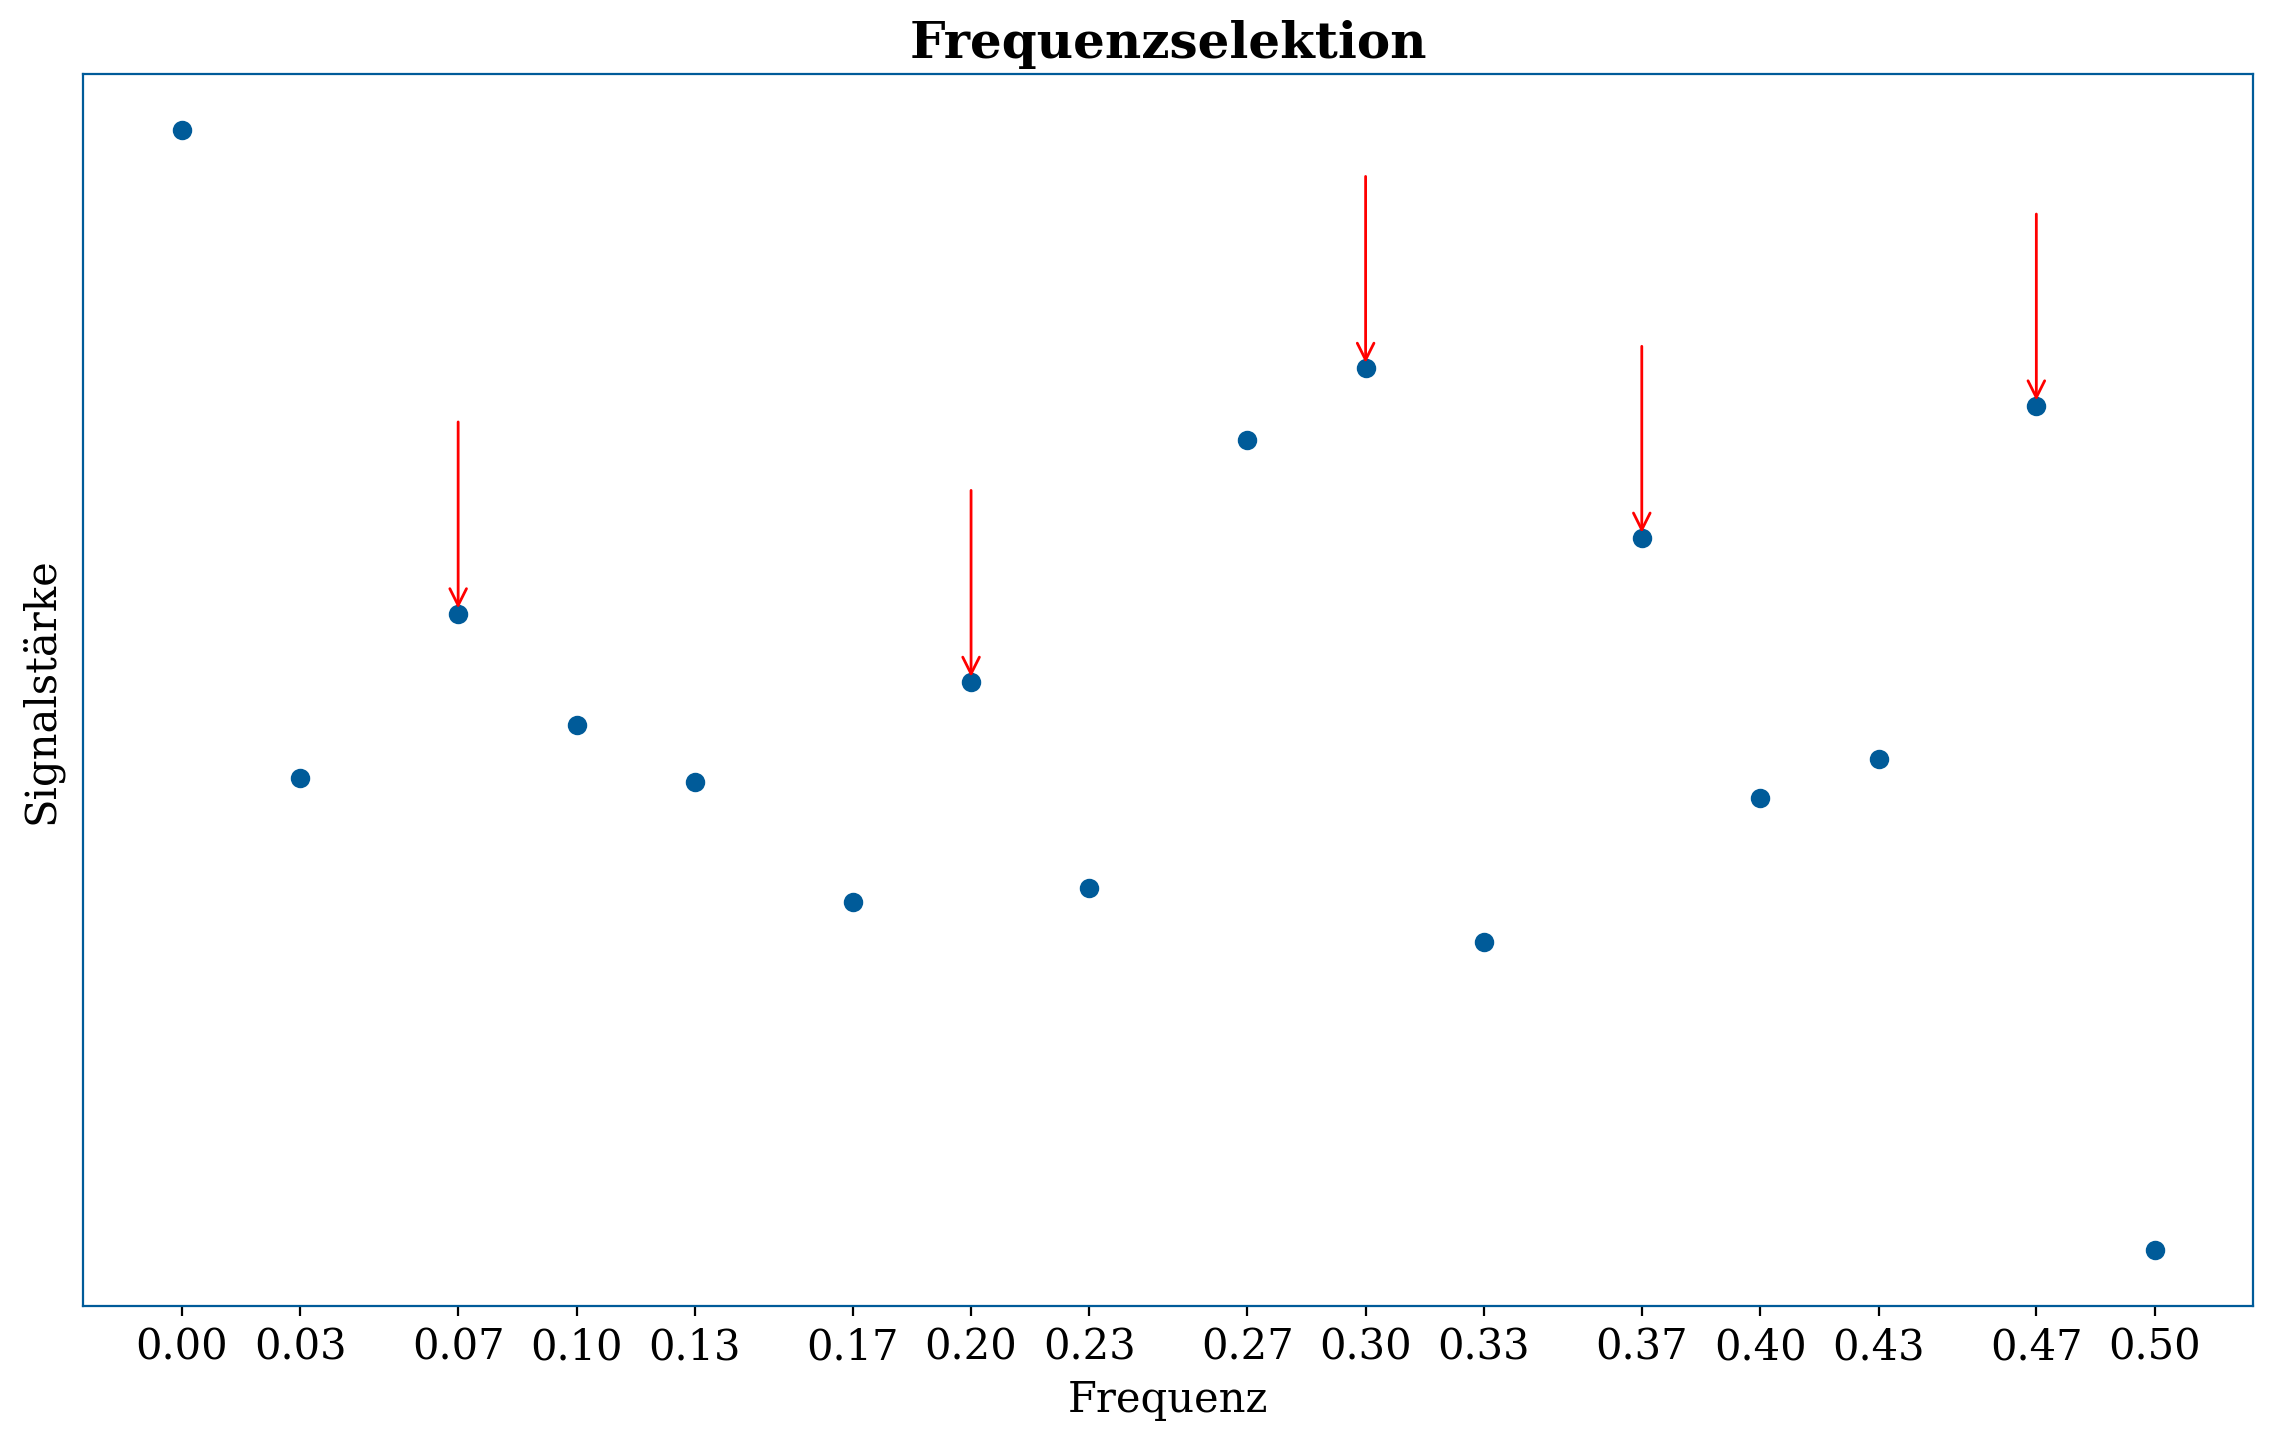
\includegraphics[width=\textwidth]{plot_frequency_selection.png}
        \caption[Spektralanalyse eines Intervalls/Fensters der STFT mit Markierung lokaler Maxima]{Spektralanalyse eines Fensters der STFT\@: Auf der x-Achse sind die Frequenzen und auf der y-Achse deren Signalstärke dargestellt. Die Pfeile markieren die lokalen Maxima als signifikant, sodass deren Frequenzen in die Datenbank einfließen. Das Reziproke einer Frequenz bedeutet, jedes wievielte Element sich wiederholt.}
        \label{fig:freq_selection}
    \end{figure}

    In \autoref{fig:freq_selection} wird dieser Sachverhalt für ein Fenster der \ac{STFT} dargestellt, also das transformierte Intervall eines numerischen Vektors. Es werden die Signalstärken für alle möglichen Frequenzen ermittelt, wobei das Reziproke einer Frequenz hier entspricht, jedes wievielte Element betrachtet wird. Bei Frequenz 0.5 wäre es also jedes $\frac{1}{0.5} = 2$te Element, hier offenbar sehr schwach ausgeprägt.

    Damit die Musikerkennung funktioniert, wird vorher eine Datenbank erstellt, welche die Periodizitäten, also die auffälligen Frequenzen, mit denen sich Elemente der Aufnahme wiederholen, der Eingabesongs mittels Hashing effizient auffindbar abspeichert, sodass der Abgleich mit einer Tonaufnahme sehr schnell und korrekt abläuft \vgl{wang}. Zudem werden hierfür aus den \ac{STFT}-Ergebnissen auch nicht alle Frequenzen verwendet, sondern nur möglichst signifikante davon. Bisher wurde das mittels der lokalen Maxima der Amplituden erreicht.

    Für die Anwendung auf Proteine werden statt des musikalischen Spektrums die numerischen Vektoren der Aminosäuresequenzen verwendet. Nun gibt es in \protfin\ zwei verschiedene Anwendungsansätze:
    \begin{enumerate}
        \item \textbf{Single-Protein:}\ \ Als Eingabe erfolgt eine einzelne Aminosäuresequenz, für die das best passende Protein gesucht wird. Je mehr Übereinstimmung herrscht, desto funktionsähnlicher sollte es sein.
        \item \textbf{Family-Matching:}\ \ Als Eingabe erfolgt eine Proteinfamilie. Die Periodizitäten, in denen sich alle Mitglieder dieser Familie ähneln, die also spezifisch für die Familie sind, werden verwendet, um Proteine zu finden, die auch in die Familie passen.
    \end{enumerate}
    \phantomsection\label{kurze_sequenzen}

    Um den Algorithmus, der von einer SHAZAM-Implementierung in Python ausgeht \autocite{blog}, für beide Ansätze auf die vergleichsweise kurzen Sequenzen von wenigen 100 Elementen abzustimmen (ein solcher Vektor für eine Sekunde Musik hätte etwa 40.000 Elemente), wurde in vorangegangenen Experimenten versucht, die Fenstergröße und die Überlappung zwischen diesen Fenstern bei der \ac{STFT} zu optimieren, beziehungsweise auch die Anzahl gewählter Frequenzen, deren Amplituden auf Periodizität hindeuten. Hierbei zeigte sich bisher allerdings eine schlechte Performanz hinsichtlich Speicher- und Laufzeitkomplexität. Die Ergebnisse dazu sind in der \autoref{fig:prev_results} dargestellt. Die Wahl der Frequenzen der \ac{STFT} Fenster und deren Abspeicherung müssen folglich noch verbessert werden.

    \begin{figure}[H]
        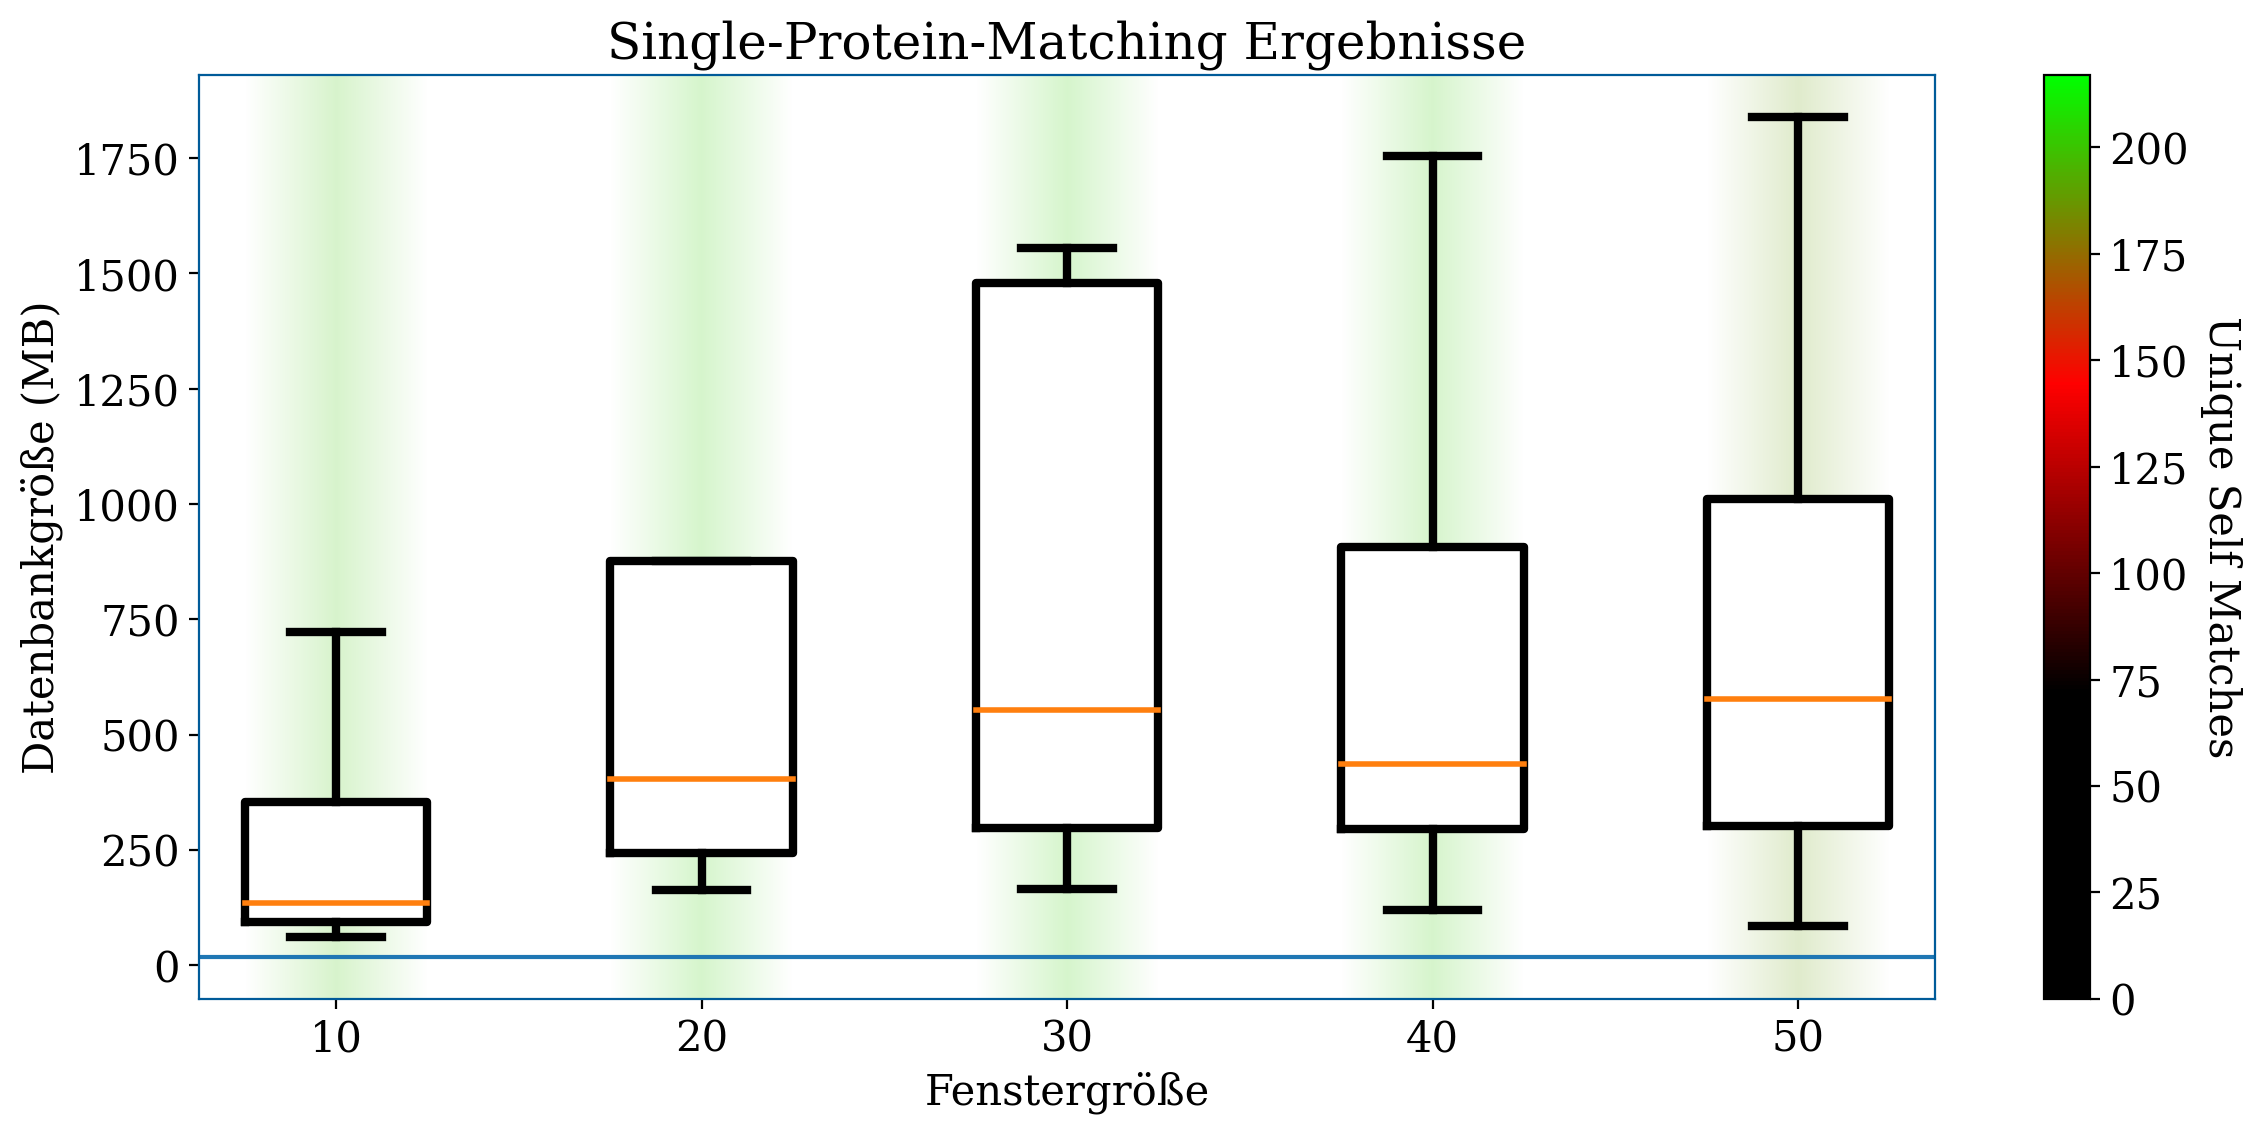
\includegraphics[width=\textwidth]{plot_previous.sp.png}
        \caption[Bisherige Ergebnisse von \protfin]{Bisherige Ergebnisse von \protfin: Überblick der Ergebnisse für die Hydrophobizität mit Verwendung verschiedener Parameter, die die \acs{STFT} betreffen (siehe \autoref{sub:durchführung}). Die Farbe stellt dar, wie viele Eingabeproteine eindeutig identifiziert wurden, die blaue Linie die Größe der Eingabedaten. Die Boxen bilden die Verteilung der Datenbankgrößen über die verschiedenen Parameterkonfigurationen ab und sind entlang der x-Achse nach der Größe eines STFT-Fensters gruppiert. Der Family-Matching Ansatz hat keine Vorergebnisse, da er erst in dieser Arbeit entwickelt wurde.}
        \label{fig:prev_results}
    \end{figure}

    Hierzu wurden in dieser Arbeit mehrere Experimente angegangen.
    \begin{enumerate}
        \item \textbf{UniRef90-Sampling:}\ \ In vergangenen Experimenten hat sich gezeigt, dass die Selektion der Frequenzen mittels lokaler Maxima (\autoref{fig:freq_selection}) suboptimal ist, weil es gelegentlich dazu kam, dass bei den kurzen Sequenzen in einem Fenster keine Maxima vorkamen. Es wurde auch versucht, für eine höhere Spezifität die Amplituden mit einzubeziehen, statt nur der Frequenzen selbst, was aber die Datenbankgröße stark erhöhte. Das UniRef90 Experiment soll beides vereinigen. Es sollen möglichst wenige aber sehr spezifische Frequenzen in einem Fenster ausgewählt werden, damit die Datenbank schlank bleibt. In diesem Experiment werden solche Fenster aus der UniRef90 Datenbank gesampelt. Sie enthält etwa 180 Mio. Aminosäuresequenzen, sodass aus jeder ein zufälliges Fenster gewählt wird. Die je Frequenz seltensten Amplituden sollen nun als Schwellwert das Wahlkriterium für eine Frequenz sein, was zu möglicherweise weniger selektierten Frequenzen mit dennoch guter Signifikanz führt.
        \item \textbf{Filter Hashes:}\ \ Ein weiterer Ansatz die Datenbankgröße zu verringern ist das Entfernen von Hashes, die sehr häufig auftreten, also folglich wenig Informationsgehalt für die Identifikation eines Proteins haben. In diesem Experiment wird daher geprüft, wie streng das erfolgen darf, um nicht zu viel Daten zu verlieren, sodass das Matching dadurch beeinträchtigt würde. 
        \item \textbf{\acl{TZ}:}\ \ Die effiziente Abspeicherung mittels Hashing basiert darauf, die Frequenzen eines Fensters mit den Frequenzen der Nachfolgefenster zu kombinieren. Die \acl{TZ} bezeichnet dabei die Anzahl betrachteter Nachfolger und ist aktuell unbeschränkt. Folglich wird hier eine Größe ermittelt, die einen guten Kompromiss zwischen der Anzahl an Kombinationen und der Genauigkeit des Matchings bildet.
        \item \textbf{Selection-Method:}\ \ Das letzte durchgeführte Experiment dieser Arbeit dient der Ermittlung einer Methode für die Frequenzselektion, die vom UniRef90-Sampling profitiert, aber die Auswahl zusätzlich reduziert. Dafür wird vor Betrachtung der Schwellwerte eine Vorselektion durchgeführt, einmal anhand der lokalen Maxima der Amplituden, dann anhand der stärksten Abweichungen der Amplituden von ihren Schwellwerten und natürlich ohne Vorselektion als Nullprobe, die nur das Sampling einbezieht.
    \end{enumerate}
    Als Trainingsdaten wird eine Referenz-Datenbank von Pflanzen-Proteinen verwendet, die in Gruppen derselben Funktion eingeordnet sind. Diese Zuordnung wurde manuell von Experten durchgeführt in sogenannte MapMan-Bins, was heißt:\\Derselbe Bin $\rightarrow$ dieselbe Funktion \autocite{mapman}\autocite{mercator}.
% section einleitung (end)